\section{Actor Model} 

In previous work~\cite{gledhill2013modelinguas}, we represented each {\em actor}, both human and autonomous component, of the WiSAR search team as a Mealy state machines as has been done in other models~\cite{bolton2013litreview}. However the Mealy state machine model does not lend itself well to workload analysis so this paper uses Moore machines\footnote{The outputs or signals from Mealy machines are based both on the inputs into the machine and the state itself,  and Moore machines restrict changes to the input to state changes.} Moore machines confine model non-determinism to state changes, which minimizes the possible sources of non-determinism and simplifies the validation process.  We augment these Moore machines with a simple form of memory.  This memory increases the computational power of the machine, but the simple form we use keeps the complexity of validation manageable.

\begin{figure}[h]
\center
\setlength{\abovecaptionskip}{1mm}
\setlength{\belowcaptionskip}{1mm}
\setlength{\textfloatsep}{1mm}
\setlength{\floatsep}{1mm}
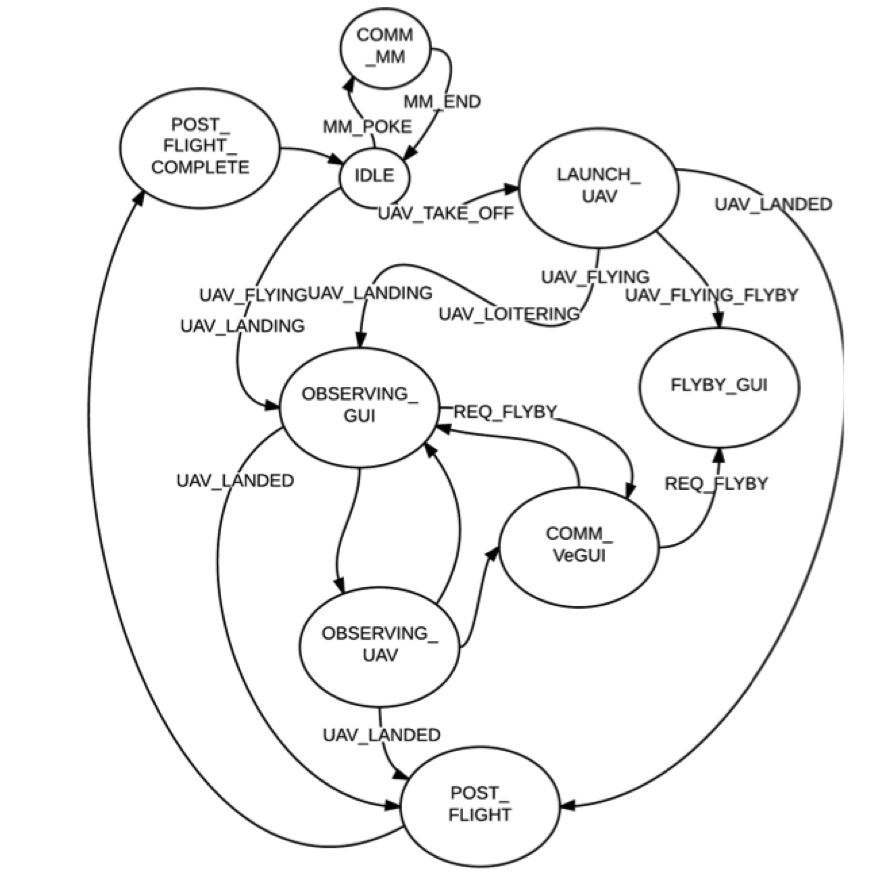
\includegraphics[height=2.4in]{DiRG.png}
\caption{Example actor model from prior work.}
\label{fig:dirg}
\end{figure}

We now present a formal description of each component of the model
\subsection{Actors}
Actors represent the human decision-makers and autonomous elements of the WiSAR team.  An actor is composed of a set of states $S$, an initial state $s_0$, a set of inputs from the environment $\Sigma_{\rm env}$, a set of inputs from other actors on the team $\Sigma_{\rm team}$, a set of outputs $\Lambda_{\rm out}$, a simple form of memory $\Omega_{\rm men}$, and a transition function that determines the next state from the inputs and memory $\delta$. Formally, we denote an actor as:
\begin{equation}
 	Actor = (S, s_0, \Sigma_{\rm env}, \Sigma_{\rm team}, \Lambda_{\rm out}, \Lambda_{\rm out} \Omega_{\rm mem},\delta)
 \label{eq:actor}
 \end{equation}
 
 \subsection{Outputs}
 An actor's output has two components: signals to other actors on a team and a {\em duration} parameter that represents the time required for the actor to complete its transition to the next state.  Thus, $\Lambda_{\rm out}=\Sigma_{\rm team} \times \Re^+$. The duration represents the relative difficulty of the
task(s) associated with the transition.  We justify this by assuming that
all tasks are performed at a constant rate, thus more difficult tasks take
longer, but note that future work should address this restrictive assumption.  
 
 \subsection{Transitions}
 
A transition is a relation on the cross product of inputs (a state, environment signal, signals from other actors, and element of memory)  with outputs (a next state, an output, and a modification to memory).  Thus,
\begin{equation}
 \delta:[S\times\Sigma_{\rm env}\times\Sigma_{\rm team}\times\Omega_{\rm mem}] \times [S\times \Sigma_{\rm team} \times \Omega_{\rm mem}], 
\end{equation} 
where we have used brackets to separate inputs from outputs.
 
Given an actor's current state, set of input signals, and memory, it is possible for multiple transitions to be possible.  This occurs because we assume that multiple environment signals or inter-actor signals may be occurring at the same time, which are all perceived by the actor since we assume perception is a parallel operation.  Thus, it is useful to explicitly note the number of possible transitions that are possible from a given state.   A transition is considered {\em enabled} when all of its input
requirements are met and {\em disabled} otherwise. 

\subsection{Current State}
When an actor is in a given state, it is useful to explicitly denote the set of enabled and disable transitions.  This allows a model-checker to use this information to create an estimate of algorithmic workload, where we assume that algorithmic workload is a function of the number of choices available to the actor.  Thus, we allow the current state to give an workload signal
 \begin{equation}
	s_0^{\rm work\  sig} = (T_{enabled}, T_{disabled}) : T_{enabled} \cap T_{disabled} = \emptyset
 \label{eq:state}
\end{equation}


\subsection{Declarative Memory }
This memory represents internal facts stored by an actor and used in decision
making.  This memory takes the form of internal variables within an actor {\sc Such as ???}

